\Askhsh{18553_SOLUTION}{1}
\begin{ylh}{1}
    \item [Ύλη από εικόνα]
\end{ylh}
\begin{wrapfigure}[24]{r}{0.5\textwidth} % Προσαρμογή του wrapfigure για να μην επικαλύπτει το κείμενο
\centering
\begin{tikzpicture}[scale=0.8]
    % Ορισμός σημείων για το Σχήμα 1 με βάση την οπτική διάταξη
    % B, Γ, Σ είναι συγγραμμικά. Α, Δ βρίσκονται σε μια παράλληλη γραμμή πάνω.
    % Α πάνω από Β, Δ πάνω από Γ.
    \tkzDefPoint(0,0){B}
    \tkzDefPoint(2,0){G} % Γάμμα
    \tkzDefPoint(4,0){S} % Σίγμα

    \tkzDefPoint(0,2){A}
    \tkzDefPoint(2,2){D} % Δέλτα

    % Σχεδίαση της κάτω γραμμής
    \tkzDrawSegment[line width=0.8pt](B,S)
    % Σχεδίαση της πάνω διακεκομμένης γραμμής
    \tkzDrawSegment[line width=0.8pt,dashed](A,D)

    % Σχεδίαση τμημάτων Α-Δ, Β-Γ, Α-Γ, Β-Δ, Δ-Σ, Γ-Σ
    \tkzDrawSegments[line width=0.8pt](A,D B,G A,G B,D D,S G,S)

    % Σχεδίαση της διακεκομμένης γραμμής από Δ παράλληλη στην ΑΣ
    % A(0,2), S(4,0) -> Κλίση = (0-2)/(4-0) = -1/2
    % Γραμμή από D(2,2) με κλίση -1/2: y-2 = -1/2(x-2) => y = -1/2x + 1 + 2 => y = -1/2x + 3
    % Σημεία για τη σχεδίαση της διακεκομμένης γραμμής
    \tkzDefPoint(-1,3.5){DashStart} % x=-1, y = -1/2(-1) + 3 = 0.5 + 3 = 3.5
    \tkzDefPoint(3,1.5){DashEnd}   % x=3, y = -1/2(3) + 3 = -1.5 + 3 = 1.5
    \tkzDrawSegment[line width=0.8pt,dashed](DashStart,DashEnd)
    
    % Ετικέτες (άλφα)
    \tkzLabelSegment[above](A,D){$\alpha$} % Οπτικά πάνω
    \tkzLabelSegment[below](B,G){$\alpha$} % Οπτικά κάτω

    % Σημεία
    \tkzDrawPoints(A,B,G,D,S)
    \tkzLabelPoint[above left](A){A}
    \tkzLabelPoint[below left](B){B}
    \tkzLabelPoint[below](G){$\Gamma$}
    \tkzLabelPoint[above right](D){$\Delta$}
    \tkzLabelPoint[below right](S){$\Sigma$}
\end{tikzpicture}
\caption*{Σχήμα για το (α)} % Λεζάντα για το σχήμα του μέρους α
\end{wrapfigure}

\Askhseis{Προτεινόμενη Λύση}

\begin{alist}
    \item [α.]
    \begin{rlist}
        \item Για να υπολογίσουμε το εμβαδό του τριγώνου $\Sigma\Delta\Gamma$ μπορούμε να πάρουμε ως βάση την πλευρά $\Delta\Gamma$, οπότε το ύψος είναι η απόσταση της κορυφής $\Sigma$ από την ευθεία $\Delta\Gamma$ που είναι ίση με $\alpha$. Άρα $\PARENS{\Sigma\Delta\Gamma} = \frac{1}{2} \cdot \alpha \cdot \alpha = \frac{\alpha^2}{2}$.
        \item Από το Πυθαγόρειο θεώρημα στο τρίγωνο $\Sigma B\Gamma$ έχουμε $\Sigma\Gamma^2 = \Sigma B^2 + B\Gamma^2$ ή $\Sigma\Gamma^2 = \alpha^2 + \alpha^2 = 2\alpha^2$ από όπου $\Sigma\Gamma = \alpha\sqrt{2}$.
    \end{rlist}

\begin{wrapfigure}[38]{r}{0.5\textwidth} % Προσαρμογή του wrapfigure για να μην επικαλύπτει το κείμενο
\centering
\begin{tikzpicture}[scale=0.8]
    % Σχήμα 2 με βάση την οπτική διάταξη
    % A, B, Γ, Σ, Σ' συγγραμμικά σε μια οριζόντια γραμμή.
    % Δ είναι πάνω από Β.
    % E και H είναι τα ίχνη των υψών από Δ.
    \tkzDefPoint(-4,0){A}
    \tkzDefPoint(-2,0){B}
    \tkzDefPoint(0,0){G} % Γάμμα
    \tkzDefPoint(2,0){S} % Σίγμα
    \tkzDefPoint(4,0){Sp} % Σίγμα'

    % Δ είναι πάνω από τη γραμμή. Ας το τοποθετήσουμε σε (1.5,3) για να επιτρέψουμε διακριτά E, H
    \tkzDefPoint(1.5,3){D} % Δέλτα

    % Σχεδίαση της κάτω γραμμής
    \tkzDrawSegment[line width=0.8pt](A,Sp)

    % Σχεδίαση τμημάτων που συνδέουν το Δ με τα σημεία στην κάτω γραμμή
    \tkzDrawSegments[line width=0.8pt,maincolor](D,A D,B D,G D,S D,Sp)

    % Σχεδίαση των υψών Δ-Ε και Δ-Η με σύμβολα ορθής γωνίας
    % Για να είναι τα E και H διακριτά και να δείχνουν ορθή γωνία με την οριζόντια γραμμή,
    % τοποθετούμε τα E και H σε διαφορετικά x-coordinates.
    % Η tkzMarkRightAngle θα τοποθετήσει το τετραγωνάκι στην γωνία που σχηματίζεται.
    \tkzDefPoint(0.5,0){E}
    \tkzDefPoint(2.5,0){H}

    % Σχεδίαση των υψών (ως τμήματα)
    \tkzDrawSegment[line width=0.8pt,secondarycolor](D,E)
    \tkzDrawSegment[line width=0.8pt,secondarycolor](D,H)
    
    % Σύμβολα ορθής γωνίας
    % Η γωνία σχηματίζεται από το τμήμα ΔΕ και την ευθεία βάσης (A-Sp) στο σημείο E.
    \tkzMarkRightAngle[fill=thirdcolor!20,size=0.2](D,E,A)
    % Η γωνία σχηματίζεται από το τμήμα ΔΗ και την ευθεία βάσης (S-G) στο σημείο H.
    \tkzMarkRightAngle[fill=thirdcolor!20,size=0.2](D,H,S)

    % Ετικέτες
    \tkzLabelPoint[above left](D){$\Delta$}
    \tkzLabelPoint[below left](A){A}
    \tkzLabelPoint[below](B){B}
    \tkzLabelPoint[below](G){$\Gamma$}
    \tkzLabelPoint[below](S){$\Sigma$}
    \tkzLabelPoint[below right](Sp){$\Sigma'$}
    \tkzLabelPoint[below](E){E}
    \tkzLabelPoint[below](H){H}
\end{tikzpicture}
\caption*{Σχήμα για το (β)} % Λεζάντα για το σχήμα του μέρους β
\end{wrapfigure}

    \item [β.]
    \begin{rlist}
        \item Τα τρίγωνα $\Sigma\Delta\Gamma$ και $\Sigma'\Delta\Gamma'$ έχουν κοινή βάση τη $\Delta\Gamma$ και ύψος ίσο με την απόσταση των παραλλήλων πλευρών $AB$ και $\Delta\Gamma$, αφού οι κορυφές τους $\Sigma$ και $\Sigma'$ βρίσκονται στην ευθεία $AB // \Delta\Gamma$. Οπότε τα τρίγωνα αυτά έχουν ίσα εμβαδά.
        \[
            \PARENS{\Sigma\Delta\Gamma} = \PARENS{\Sigma'\Delta\Gamma'} = \frac{1}{2} \cdot \alpha \cdot \alpha = \frac{\alpha^2}{2}
        \]
        \item Από το σημείο $\Gamma$ έχουμε το κάθετο τμήμα $\Gamma B$ προς την ευθεία $AB$ και τα πλάγια $\Gamma\Sigma$ και $\Gamma\Sigma'$. Τα ίχνη $\Sigma$ και $\Sigma'$ των πλαγίων τμημάτων $\Gamma\Sigma$ και $\Gamma\Sigma'$ αντιστοιχεί είναι τέτοια ώστε οι αποστάσεις τους από το ίχνος $B$ του καθέτου $\Gamma B$ να είναι άνισες και συγκεκριμένα $B\Sigma' > B\Sigma$, οπότε και τα αντίστοιχα πλάγια είναι ομοίως άνισα δηλαδή $\Gamma\Sigma' > \Gamma\Sigma$.
        \item Η απόσταση του σημείου $\Delta$ από την ευθεία $\Sigma\Gamma$ είναι ίση με το μήκος του τμήματος $\Delta E$ και η απόσταση του σημείου $\Delta$ από την ευθεία $\Sigma'\Gamma'$ είναι ίση με το μήκος του τμήματος $\Delta H$. Ισχύει $\PARENS{\Sigma'\Delta\Gamma'} = \frac{1}{2} \cdot \Sigma'\Gamma' \cdot \Delta H$ και $\PARENS{\Sigma\Delta\Gamma} = \frac{1}{2} \cdot \Sigma\Gamma \cdot \Delta E$.
        Δείξαμε στο ερώτημα βi) ότι τα τρίγωνα $\Sigma'\Delta\Gamma'$ και $\Sigma\Delta\Gamma$ είναι ισεμβαδικά οπότε θα έχουμε:
        \[
            \frac{1}{2} \cdot \Sigma'\Gamma' \cdot \Delta H = \frac{1}{2} \cdot \Sigma\Gamma \cdot \Delta E \text{ ή } \Sigma'\Gamma' \cdot \Delta H = \Sigma\Gamma \cdot \Delta E
        \]
        και επειδή $\Sigma'\Gamma' > \Sigma\Gamma$ θα έχουμε $\Delta E > \Delta H$. Δηλαδή η απόσταση του σημείου $\Delta$ από την ευθεία $\Sigma'\Gamma'$ είναι μικρότερη από την απόσταση του σημείου $\Delta$ από την ευθεία $\Sigma\Gamma$.
    \end{rlist}
\end{alist}